\documentclass{beamer}

\usetheme{CambridgeUS}  % Select your favorite theme
\usepackage{tikz}
\usetikzlibrary{positioning}


\title{Penrose Tilings from Pentagrids}
\author{Your name(s) goes here}
\institute{SEGL Seminars}
\date{\today}

\begin{document}

\begin{frame}
\titlepage
\end{frame}

\section{Section 1}


\begin{frame}
    \frametitle{Summary}
    \begin{center}
        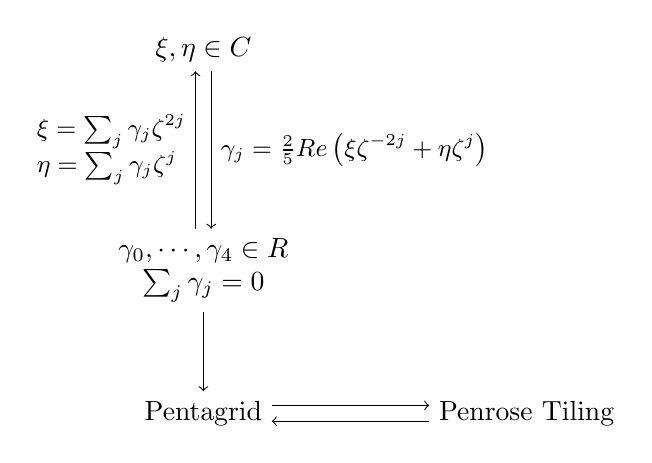
\begin{tikzpicture}[node distance=4cm, auto]
            % 노드 생성
            \node (pentagrid) {Pentagrid};
            \node (penrose) [right=2cm of pentagrid] {Penrose Tiling};
            \node (gamma) [above=1cm of pentagrid, align=center] {$\gamma_0, \cdots, \gamma_4 \in \mathbb{R}$ \\ $\sum_j \gamma_j = 0$};
            \node (xi) [above=2cm of gamma] {$\xi, \eta \in \mathbb{C}$};
            
            % 화살표 그리기
            \draw[->] (gamma) -- (pentagrid);
            \draw[->] ([xshift=-0.1cm]gamma.north) -- node[midway, left, align=left] {\small{$\xi = \sum_{j} \gamma_j \zeta^{2j}$} \\ \small{$\eta = \sum_{j} \gamma_j \zeta^{j}$}} ([xshift=-0.1cm]xi.south);
            \draw[->] ([xshift=0.1cm]xi.south) -- node[midway, right] {\small{$\gamma_j = \frac{2}{5} \text{Re}\left(\xi \zeta^{-2j} + \eta \zeta^{j}\right)$}} ([xshift=0.1cm]gamma.north);
              
            % 위쪽 화살표 그리기
            \draw[->] ([yshift=0.1cm]pentagrid.east) -- ([yshift=0.1cm]penrose.west);
              
            % 아래쪽 화살표 그리기
            \draw[->] ([yshift=-0.1cm]penrose.west) -- ([yshift=-0.1cm]pentagrid.east);
        \end{tikzpicture}
    \end{center}
\end{frame}


\begin{frame}
\frametitle{Frame 2}

Let
$$K_j\left(z\right) = \left\lceil\text{Re}\left(z \zeta^{-j}\right) + \gamma_j\right\rceil$$

. For each point of intersection of pentagrids, $z$, we assign a vector 
$$\left(K_0\left(z\right), \cdots, K_4\left(z\right)\right)$$
. If z is an intersection point of $i$-th and $j$-th pentagrid,

\end{frame}

\begin{frame}
\Huge{\centerline{Thank You}}
\end{frame}

\end{document}
